% This file should be compiled with V2.5 of "sig-alternate.cls" May 2012
% This file has been modified by Brian Chen (bchen12@ucsc.edu) for the purpose of simplifying the sections
%
% This example file demonstrates the use of the 'sig-alternate.cls'
% V2.5 LaTeX2e document class file. It is for those submitting
% articles to ACM Conference Proceedings WHO DO NOT WISH TO
% STRICTLY ADHERE TO THE SIGS (PUBS-BOARD-ENDORSED) STYLE.
% The 'sig-alternate.cls' file will produce a similar-looking,
% albeit, 'tighter' paper resulting in, invariably, fewer pages.
%
% ----------------------------------------------------------------------------------------------------------------
% This .tex file (and associated .cls V2.5) produces:
%       1) The Permission Statement
%       2) The Conference (location) Info information
%       3) The Copyright Line with ACM data
%       4) NO page numbers
%
% as against the acm_proc_article-sp.cls file which
% DOES NOT produce 1) thru' 3) above.
%
% Using 'sig-alternate.cls' you have control, however, from within
% the source .tex file, over both the CopyrightYear
% (defaulted to 200X) and the ACM Copyright Data
% (defaulted to X-XXXXX-XX-X/XX/XX).
% e.g.
% \CopyrightYear{2007} will cause 2007 to appear in the copyright line.
% \crdata{0-12345-67-8/90/12} will cause 0-12345-67-8/90/12 to appear in the copyright line.
%
% ---------------------------------------------------------------------------------------------------------------
% This .tex source is an example which *does* use
% the .bib file (from which the .bbl file % is produced).
% REMEMBER HOWEVER: After having produced the .bbl file,
% and prior to final submission, you *NEED* to 'insert'
% your .bbl file into your source .tex file so as to provide
% ONE 'self-contained' source file.
%
% ================= IF YOU HAVE QUESTIONS =======================
% Questions regarding the SIGS styles, SIGS policies and
% procedures, Conferences etc. should be sent to
% Adrienne Griscti (griscti@acm.org)
%
% Technical questions _only_ to
% Gerald Murray (murray@hq.acm.org)
% ===============================================================
%
% For tracking purposes - this is V2.0 - May 2012
% Custom Modified Version - November 2013

\documentclass{sig-alternate-05-2015}
%\RequirePackage[pdftex]{hyperref}
\usepackage{comment}
\usepackage{graphicx}
\usepackage[autostyle]{csquotes}
\usepackage{subfigure}

\newcommand{\fixme}[1]{{\Large FIXME:} {\bf #1}}
\newcommand{\todo}[1]{{\bf TODO: {#1}}\\}
\newcommand{\note}[1]{{\bf Note:} \{#1\}\\}
\newcommand{\comm}[1]{\small{\it{  //{#1}}}}


% --- Author Metadata here ---
\conferenceinfo{ICCAD}{International Conference on Computer-Aided Design}
%\CopyrightYear{2007} % Allows default copyright year (20XX) to be over-ridden - IF NEED BE.
%\crdata{0-12345-67-8/90/01}  % Allows default copyright data (0-89791-88-6/97/05) to be over-ridden - IF NEED BE.
% --- End of Author Metadata ---

\title{OpenRAM: An Open-Source Memory Compiler\\
\vspace{-0.5cm}\center{\normalsize{Invited Paper}}}
%\titlenote{Some Copyright info about OpenRAM??????}}

\numberofauthors{1}
\author{
  %% TO DAC: Guthaus, Stine, Ataei, Chen, Wu, Sarwar
\alignauthor Matthew R. Guthaus$^1$, James E. Stine$^2$, Samira Ataei$^2$, \\Brian Chen$^1$, Bin Wu$^1$, Mehedi Sarwar$^2$ \\
\affaddr{$^1$ Department of Computer Engineering, University of California Santa Cruz, Santa Cruz, CA 95064}\\
\affaddr\{mrg, bchen12, bwu8\}@ucsc.edu \\ 
\affaddr{$^2$ Electrical and Computer Engineering Department, Oklahoma State University, Stillwater, OK 74078}\\
\affaddr\{james.stine, ataei, mehedis\}@okstate.edu}
 
 %% \alignauthor Matthew Guthaus, Brian Chen, Bin Wu \\
 %%     \affaddr{Department of Computer Engineering} \\
 %%     \affaddr{University of California Santa Cruz} \\
 %%     \affaddr{Santa Cruz, CA 95064, USA} \\
 %%     \affaddr{\{mrg,bchen12,bwu8\}@ucsc.edu}
 %% \and
 %% \alignauthor James Stine, Samira Ataei, Mehedi Sarwar \\
 %%     \affaddr{Electrical and Computer Engineering Department} \\
 %%     \affaddr{Oklahoma State University} \\
 %%     \affaddr{Stillwater, OK 74078} \\
 %%     \affaddr{\{james.stine,ataei,XXXX\}@okstate.edu}
 %%} 


\begin{document}

\CopyrightYear{2016} 
\setcopyright{acmlicensed}
\conferenceinfo{ICCAD '16,}{November 07 - 10, 2016, Austin, TX, USA}
\isbn{978-1-4503-4466-1/16/11}\acmPrice{\$15.00}
\doi{http://dx.doi.org/10.1145/2966986.2980098}
\maketitle

\begin{abstract}
Computer systems research is often inhibited by the availability of
memory designs. Existing Process Design Kits (PDKs) frequently lack
memory compilers, while expensive commercial solutions only provide
memory models with immutable cells, limited configurations, and
restrictive licenses. Manually creating memories can be time consuming
and tedious and the designs are usually inflexible. This paper
introduces OpenRAM, an open-source memory compiler, that provides a
platform for the generation, characterization, and verification of
fabricable memory designs across various technologies, sizes, and
configurations. It enables research in computer architecture,
system-on-chip design, memory circuit and device research, and
computer-\allowbreak aided design.
\end{abstract}


%\category{J.6}{COMPUTER-AIDED ENGINEERING}{\\Computer-aided design (CAD)}
%\terms{Design, Algorithms}
%\keywords{OpenRAM, Memory Compiler, Open-source}

\section{Introduction}
\label{sec:introduction}

% why memory compilers are important
Static Random Access Memories (SRAMs) have become a standard component
embedded in all System-on-Chip (SoC), Application-Specific Integrated
Circuit (ASIC), and micro-processor designs. Their wide application
leads to a variety of requirements in circuit design and memory
configuration. However, manual design is 
too time consuming. The
regular structure of memories leads well to automation that produces
size and configuration variations quickly, but developing this with
multiple technologies and tool methodologies is challenging. In
addition, memory designs play a significant role in overall system
performance and costs, so optimization is important. Thus, a memory
compiler is a critical tool.

% why academics need memory compilers
Most academic ICs design methodologies are limited by the availability
of memories. Many standard-cell Process Design Kits (PDKs) are
available from foundries and vendors, but these PDKs frequently do not
come with memory arrays or memory compilers. If a memory compiler is
freely available, it often only supports a generic process technology
that is not fabricable.  Due to academic funding restrictions,
commercial industry solutions are often not feasible for
researchers. In addition, these commercial solutions are limited in
customization of the memory sizes and specific components of the
memory. PDKs may have the options to request \enquote{black box}
memory models, but these are also not modifiable and have limited
available configurations. These restrictions and licensing issues make
comparison and experimentation with real world memories impossible.

% manually designing is time consuming
Academic researchers are able to design their own custom memories, but
this can be a tedious and time-consuming task and may not be the intended
purpose of the research. Frequently, the memory design is the bare
minimum that the research project requires,
and, because of this, the memory designs are often inferior and are not
optimized. In memory research, peripheral circuits are often not
considered when comparing memory performance and density. The
lack of a customizable compiler makes it difficult for researchers to
prototype and verify circuits and methodologies beyond a single row or
column of memory cells.

% what are the goals of OpenRAM
The OpenRAM project aims to provide an open-source memory compiler
development framework for memories. It provides reference circuit and
physical implementations in a generic $45$nm technology and fabricable
Scalable CMOS (SCMOS), but it has also been ported to several
commercial technology nodes using a simple technology file. OpenRAM
also includes a characterization methodology so that it can generate
the timing and power characterization results in addition to circuits and
layout while remaining independent of specific commercial tools. Most
importantly, OpenRAM is completely user-modifiable since all source
code is open source at:
\begin{center}
\url{https://openram.soe.ucsc.edu/}
\end{center}

The remainder of this paper is organized as follows:
Section~\ref{sec:background} provides a background on previous memory
compilers. Section~\ref{sec:architecture} presents the reference
memory architecture in OpenRAM. Section~\ref{sec:implementation}
specifically introduces the implementation and main features of the
OpenRAM memory compiler. In Section~\ref{sec:results}, an analysis of
the area, timing and power is shown for different sizes and
technologies of memory. Finally, the paper is summarized in
Section~\ref{sec:conclusions}.

\section{Background}
\label{sec:background}
% brief origin/background of memory compilers

% Existence of memory compilers from the beginning
Memory compilers have been used in Electronic Design Automation (EDA)
design flows to reduce the design
time long before contemporary
compilers~\cite{broderson:sicompiler,johannsen:blocks}.
However, these compilers were generally not portable as they were 
nothing more
than quick scripts to aid designers. Porting to a new technology
essentially required rewriting the scripts. However, the increase in
design productivity when porting designs between technologies has led to
more research on memory array
compilers~\cite{cabe:flexible,huang:array,poechmueller:array,Xu:2007}.

% Reason why compilers evolved to today's current version
As technology entered the Deep Sub-Micron (DSM) era, memory designs
became one of the most challenging parts of circuit design
due to decreasing static noise margins (SNM), increasing fabrication
variability, and increasing leakage power consumption. 
This increased the complexity of memory compilers dramatically as they had to
adapt to the ever-changing technologies. Simultaneously, design
methodologies shifted from silicon compilers to standard cell place
and route methods which required large optimized libraries. During
this time, industry began using third-party suppliers of standard cell
libraries and memory compilers that allowed their reuse to amortize
development costs. These next-generation memory compilers provided
silicon-verification that allowed designers to focus on their new
design contribution rather than time-consuming tasks such as memory
generation.

% Commercial industry memory compilers' description and cost
Contemporary memory compilers have been widely used by industry, but
the internal operation is typically hidden. Several prominent
companies and foundries have provided memory compilers to their
customers. These memory compilers usually allow customers to view
front-end simulation, timing/power values, and pin locations after a
license agreement is signed. Back-end features such as layout are
normally supplied directly to the fab and are only given to the user
for a licensing fee.

% Examples of commercial compilers' drawbacks
Specifically, Global Foundries offers front-end PDKs for free, but not
back-end detailed views~\cite{globalfoundries:2015}.  Faraday
Technologies provides a \enquote{black box} design kit where users do
not know the details of the internal memory
design~\cite{faraday:2015}. Dolphin Technology offers closed-source
compilers which can create RAMs, ROMs, and CAMs for a variety of
technologies~\cite{dolphin:2015}. The majority of these commercial
compilers do not allow the customer to alter the base design, are
restricted by the company's license, and usually require a fee. This
makes them virtually unavailable and not useful for many academic
research projects.

% Describe the problem (no free open-source that is widely distributed)
In addition to memory compilers provided by industry, various research
groups have released scripts to generate memories. However, these
designs are not silicon verified and are usually only composed of
simple structures.  For example, FabMem is able to
create small arrays, but it is highly dependent on the Cadence design
tools~\cite{fabmem:2010}. The scripts do not provide any characterization capability
and cannot easily integrate with commercial place and route tools.

% Industry's attempt to provide academia a memory compiler
Another recent, promising solution for academia is the Synopsys
Generic Memory Compiler (GMC)~\cite{Goldman:2014}. The software is
provided with sample generic libraries such as Synopsys' $32$/$28$nm and
$90$nm abstract technologies and can generate the entire SRAM for these
technologies. The GMC generates GDSII layout data, SPICE netlists,
Verilog and VHDL models, timing/power libraries, and DRC/LVS
verification reports. GMC, however, is not recommended for
fabrication since the technologies it supports are not real. Its sole
purpose is to aid students in VLSI courses to learn about using
memories in design flows.

% Academia's' attempts at a memory compiler
There have been multiple attempts by academia to implement a memory
compiler that is not restricted: the Institute of
Microelectronics' SRAM IP Compiler~\cite{Xu:2007}, School of
Electronic Science and Engineering at Southeast University's Memory IP
Compiler~\cite{Chen:2012}, and Tsinghua University's Low Power SRAM
Compiler~\cite{Wu:2010}. These are all methodologies and design flows
for a memory compiler, but there are no public releases.

% State what we are looking for in academia. -- duplicate from introduction
%% With all these attempts, there still isn't a complete solution for
%% academia's research needs.  Researchers need a memory compiler that is
%% open-source, platform- and tool-portable, technology independent, and
%% can generate fabricable memory designs.

                                                     

\section{Architecture}
\label{sec:architecture}

% Overview of SRAM blocks
The OpenRAM SRAM architecture is based on a bank of memory cells
with peripheral circuits and control logic as illustrated in
Figure~\ref{fig:structure}. These are further refined into eight major
blocks: the bit-cell array, the address decoder, the word-line drivers,
the column multiplexer, the pre-charge circuitry, the sense amplifier,
the write drivers, and the control logic.

\begin{figure}[tb]
\centering
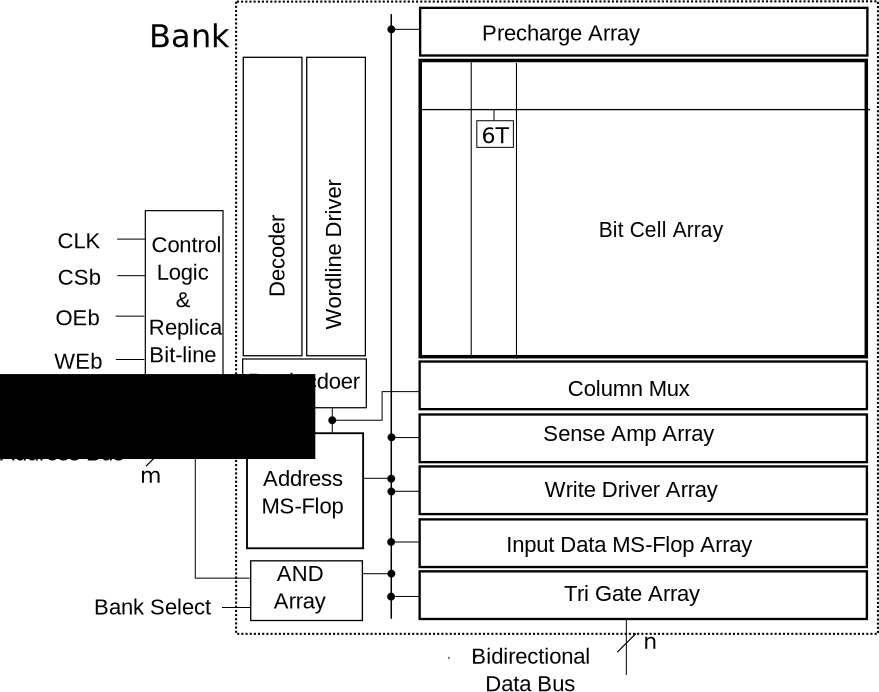
\includegraphics[width=8cm]{./figs/sram_structure.pdf}
\caption{An OpenRAM SRAM consists of a bit-cell array along with decoder, 
  reading and writing circuitry and control logic timed with a replica
  bit-line.
\label{fig:structure}}
\end{figure}

% we don't implement these yet, so don't give a tutorial on them
%% General memories and Register Files (RF) are both examples of what an
%% memory compiler can generate. General memories usually have shared
%% read/write ports whereas RFs typically have separate ports. All of
%% these options are permitted through the use of different types of
%% memory cells such as 6, 8, and 12 transistor (T) cells which contains
%% 1-4 access transistor pairs and their associated bit-lines. Some basic
%% memory array options are available below:
%% \begin{itemize}
%% \setlength{\itemsep}{0pt} \setlength{\parskip}{0pt}
%% \item Standard 6T cell for single-port memory
%% \item Dual-port 8T cell for dual-port memory or separate read/write ports
%% \item Four-port 12T cell for dual separate read/write ports
%% \item Custom sense amplifier designs for different performances
%% \item Different types of address decoders for different performances
%% \end{itemize}

\begin{figure*}[tb]
\centering
\subfigure[Read operation timing]{
\includegraphics[width = 8cm]{figs/timing_read.pdf}
\label{fig:timing_read}}
\subfigure[Write operation timing]{
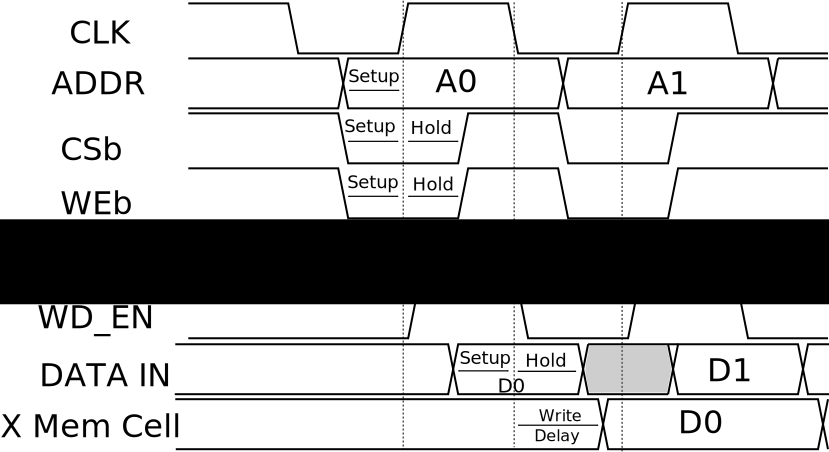
\includegraphics[width = 8cm]{figs/timing_write.pdf}
\label{fig:timing_write}}
\caption{OpenRAM uses a synchronous SRAM interface using a system
  clock (clk) along with control signals: output enable (OEb), chip
  select (CSb) and write enable (WEb).}
\label{fig:timing}
\end{figure*}

{\bf Bit-cell Array:} In the initial release of OpenRAM, the $6$T cell
is the default memory cell because it is the most commonly used cell
in SRAM devices. $6$T cells are tiled together with abutting word- and
bit-lines to make up the memory array.  The bit-cell array's aspect
ratio is made as square as possible using multiple columns of data
words. The memory cell is a custom designed library cell for each technology.
Other types of memory cells, such as $7$T, $8$T, and $10$T cells, can be used
as alternatives to the $6$T cell.

{\bf Address Decoder:} The address decoder takes the row address bits
as inputs and asserts the appropriate word-line so that the correct
memory cells can be read from or written to. The address decoder is
placed to the left of the memory array and spans the array's vertical
length. Different types of decoders can be used such as an included
dynamic NAND decoder, but OpenRAM's default option is a hierarchical CMOS
decoder.

{\bf Word-Line Driver:} Word-line drivers are inserted between the
address decoder and the memory array as buffers. The word-line drivers
are sized based on the width of the memory array so that they can drive
the row select signal across the bit-cell array.

{\bf Column Multiplexer:} The column multiplexer is an optional block
that uses the lower address bits to select the associated word in a
row. The column mux is dynamically generated and can be omitted or can
have 2 or 4 inputs. Larger column muxes are possible, but are not
frequently used in memories. There are options for a multi-level tree
mux as well.

{\bf Bit-line Precharge:} This circuitry pre-charges
the bit-lines during the first phase of the clock for read
operations. The precharge circuit is placed on top of every column in
the memory array and equalizes the bit-line voltages so that the
sense amplifier can sense the voltage difference between the two
bit-lines.

{\bf Sense Amplifier:} A differential sense amplifier is used to sense
the voltage difference between the bit-lines of a memory cell while a
read operation is performed.  The sense amplifier uses a bit-line
isolation technique to increase performance. The sense amplifier
circuitry is placed below the column multiplexer or the memory
array if no column multiplexer is used. There is one sense amplifier for
each output bit.

{\bf Write Driver:} The write drivers send the input data signals onto the
bit-lines for a write operation. The write drivers are tri-stated
so that they can be placed between the column multiplexer/memory array
and the sense amplifiers. There is one write driver for each input
data bit.

%% \subsubsection{Bit-cell and Bit-cell Array}
%% A bit-cell class is provided to instantiate the custom designed memory
%% cell located in the technology directory. Then the bit-cell array class
%% will take the single bit-cell instance to dynamically generate the
%% memory array. Using the functionality of GdsMill, we can rotate and/or
%% mirror an instance. Doing so, will allow us to abut the power rails.

%% \subsubsection{Address Decoder}
%% The hierarchical decoder is the default row address decoder that is
%% used in OpenRAM. The hierarchical decoder is dynamically generated
%% using the inverter and NAND gates with the help of basic shapes. The
%% height of each decoder row will match the height of the memory cell so
%% that the power rails can be abutted. OpenRAM also provides a NAND
%% decoder as an alternative. NAND decoder uses NMOS and PMOS transistors
%% created by ptx class. User can define type of the decoder in the
%% configuration file.

%% \subsubsection{Word-line Driver}
%% The word-line driver will be a column of alternating "mirrored"
%% inverters instances that is used to drive the signal to access the
%% memory cells in the row. The inverters will be sized accordingly
%% depending on the size of the memory array.

%% \subsubsection{Column Multiplexer}
%% The column multiplexer is an optional block that is used depending on
%% the size of the memory array. By generating an instance of a 1-1
%% multiplexer, we can then tile them to create bigger multiplexers such
%% as 2-1, 4-1, etc. OpenRAM has two options for column multiplexing.
%% Single-level-column-mux is the default column multiplexer but user can
%% choose Tree-Column-Mux in configuration file.  Both multiplexers use
%% transistors created by ptx class.

%% \subsubsection{Precharge and Precharge Array}
%% The precharge circuitry is dynamically generated using the transistor
%% instances and various basic shapes. The precharge class dynamically
%% generates an instance for a single column. The precharge array class
%% takes that instance and tiles them horizontally to match the number of
%% columns in the memory array. The width of the precharge cell is
%% determined by the width of the user-created memory cell.

%% \subsubsection{Sense Amplifier and Sense Amplifier Array}
%% The sense amplifier is user-designed analog circuit that is placed in
%% the technology directory. The sense amplifier class instantiates the
%% library cell and the sense amplifier array takes that instance to
%% create a horizontal array matching the number of output bits for the
%% memory. When designing this library cell, the user should match this
%% cell's width and bit-lines to the memory cell's.

%% \subsubsection{Write Driver and Write Driver Array}
%% Similar to the precharge classes, the write driver class will generate
%% an instance for a single bit and the write driver array will tile them
%% horizontally to match the number of input bits for the memory. The
%% write drivers will be dynamically sized accordingly based on the size
%% of the memory array.

%% \subsubsection{Control Logic}
%% There will be a control logic module that will arrange the
%% master-slave flip-flops and the logic associated with the control
%% signals into a single design. Flip-flops are used to drive the control
%% signals and standard library cells such as NAND and NOR gates will be
%% used for the logic.  A RBL is also generated using parameterized gates
%% and Replica Cell (RC). RC is a 6T SRAM memory cell which is hard-wired
%% to store a zero in order to discharge the RBL and generate the sense
%% amplifier enable signal in read mode.

%% \subsubsection{Additional Arrays}
%% In addition to the eight main blocks, there are helper modules that
%% help simplify the designs in the eight main blocks. We have a
%% flip-flop array class that takes the custom designed master-slave
%% flip-flop library cell to create a tiled array.  We also have the
%% tri-state array class that will generate the array of tri-states for
%% the DATA bus.

% Overview of signal inputs and timing
{\bf Control Logic:} The OpenRAM SRAM architecture incorporates a
standard synchronous memory interface using a system clock (clk). The
control logic uses an externally provided, active-low output enable
(OEb), chip select (CSb), and write enable (WEb) to combine multiple
SRAMs into a larger structure. Internally, the OpenRAM compiler can
have $1$, $2$, or $4$ memory banks to amortize the area/power cost of
control logic and peripheral circuitry.

All of the input control signals are stored using master-slave (MS)
flip-flops (FF) to ensure that the signals are valid for the entire
clock cycle. During a read operation, data is available after the
negative clock edge (second half of cycle) as shown in
Figure~\ref{fig:timing_read}. To avoid dead cycles which degrade
performance, a Zero Bus Turn-around (ZBT) technique is used in OpenRAM
timing. The ZBT enables higher memory throughput since there are no
wait states. During ZBT writes, data is set up before the negative
clock edge and is captured on the negative edge. Figure~\ref{fig:timing_write}
shows the timing for input signals during the write operation.

The internal control signals are generated using a replica bit-line (RBL)
structure for the timing of the sense amplifier enable and output
data storage~\cite{RBL:1998}. The RBL turns on the sense amplifiers 
at the exact time in presence of process variability in sub-$100$nm 
technologies.


\section{Software Implementation}
\label{sec:implementation}

OpenRAM is implemented using object-oriented data structures in the
Python programming language. The top-level executable is
\verb|openram.py| which parses input arguments, creates the memory and
saves the output.


\subsection{Design Hierarchy}
\label{sec:design}

All modules in OpenRAM are derived from the \verb|design| class in
\verb|design.py|. The design class is a data structure that consists
of a spice netlist, a layout, and a name. The spice netlist
capabilities are inherited from the \verb|hierarchy_spice| class while
the layout capabilities are inherited from the \verb|hierarchy_layout|
class.  The only additional function in design.py is \verb|DRC_LVS()|,
which performs a DRC/LVS check on the module.


\begin{figure}[htb]
\centering
\includegraphics[width=10cm]{./figs/class_hierarchy.pdf}
\caption{Class hierarchy}
\label{fig:class_hierarchy}
\end{figure}

\subsubsection{Spice Hierarchy}

The spice hierarchy is stored in the \verb|spice| class in
\verb|hierarchy_spice.py|.  When the design class is initialized for a
module, a data structure for the spice hierarchy is created.  The
spice data stucture name becomes the name of the top-level subcircuit
definition for the module.  The list of pins for the module are added
to the subcircuit definition by using the \verb|add_pin()| function.
The \verb|add_mod()| function adds an instance of a
module/library\_cell/parameterized\_cell as a subcircuit to the
top-level structure.  Each time a sub-module has been added to the
hierarchy, the pins of the sub-module must be connected using the
\verb|connect_pins()| function.  It is important to note that the pins
must be listed in the same order as they were added to the submodule.
Also, an assertion error will occur if there is a mismatch in the
number of net connections.  The \verb|spice| class also contains
functions for reading or writing spice files:
\begin{itemize}
\item \verb|sp_read():| this function is used to read in spice
  netlists and parse the inputs defined by the ``subckt'' definition.
\item \verb|sp_write():| this function creates an empty spice file in
  write mode and calls \verb|sp_write_file()|.
\item \verb|sp_write_file():| this function recursively writes the
  modules and sub-modules from the data structure into the spice file
  created by \verb|sp_write()|.
\end{itemize}

\subsubsection{Layout Hierarchy}

The layout hierarchy is stroed in the \verb|layout| class in
\verb|hierarchy_layout.py|.  When the design class is initialized for
a module, a data structure for the layout hierarchy is created.  The
layout data structure has two main components: a structure for the
instances of sub-modules contained in the layout, and a structure for
the objects (such as shapes, labels, etc...) contained in the layout.
The functions included in the \verb|layout| class are:
\begin{itemize}
\item \verb|def add_inst(self,name,mod,offset,mirror):| adds an
  instance of a physical layout (library cell, module, or
  parameterized cell) to the module. The input parameters are :
  \begin{description}
  \item[name] - name for the instance.
  \item[mod] - the associated spice module.
  \item[offset] - the x-y coordinates, in microns, where the instance
    should be placed in the layout.
  \item[mirror] - mirror or rotate the instance before it is added to
    the layout.  Accepted values for mirror are:
    \verb|"R0", "R90", "R180", "R270"|  $^\ast$Currently, only ``R0'' works.\\
    \verb|"MX" or "x", "MY" or "y", "XY" or "xy"| (``xy'' is
    equivalent to ``R180'')
  \end{description}
\item \verb|add_rect(self,layerNumber,offset,width,height):| adds a
  rectangle to the module's layout. The inputs are:
  \begin{description}
  \item[layernumber] - the layer that the rectangle is to be drawn in.
  \item[offset] - the x-y coordinates, in microns, where the
    rectangle's origin will be placed in the layout.
  \item[width] - the width of the rectangle, can be positive or
    negative value.
  \item[height] - the height of the rectangle, can be positive or
    negative value.
  \end{description}
\item \verb|add_label(self,text,layerNumber,offset,zoom):| adds a
  label to the layout. The inputs are:
  \begin{description}
  \item[text] - the text for the label
  \item[layernumber] - the layer that the label is to be drawn in .
  \item[offset] - the x-y coordinates, in microns, where the label
    will be placed in the layout.
  \item[zoom] - magnification of the label (ex: ``1e9'').
  \end{description}
\item \verb|add_path(self,layerNumber,coordinates,width):| this
  function is under construction...
\item \verb|gds_read():| reads in a GDSII file and creates a
  \verb|VlsiLayout()| class for it.
\item \verb|gds_write():| writes the entire GDS of the object to a
  file by gdsMill \verb|vlsiLayout()| class and calling the
  \verb|gds2writer()| (see Sections~\ref{sec:vlsilayout}
  and~\ref{sec:gdsmill}.
\item \verb|gds_write_file():| recursively the instances and objects
  in layout data structure to the gds file.
\item \verb|pdf_write():| this function is under construction...
\end{itemize}


\subsection{Creating a New Design Module}
\label{sec:new_design}

Each module in the SRAM is its own Python class, which contains a
design class, or data structure, for the layout and spice.  The
\verb|design| class (\verb|design.py|) is initialized within the
module class, subsequently creating separate data structurse to hold
the layout (\verb|hierarchy_layout|) and spice
(\verb|hierarchy_spice|) information.  By having a class for each
module, it is very easy to instatiate instances of the modules in any
level of the hierarchy.  Follow these guidelines when creating a new
module:


\begin{itemize}
\item Derive your class from the design module:
\begin{verbatim}
class bitcell_array(design.design):
\end{verbatim}
\item Always use the python constructor \verb|__init__| method so that
  your class is initialized when an object of the module is
  instatiated. The module parameters should also be declared:
\begin{verbatim}
def __init__(self, cols, rows): 
\end{verbatim}
\item In the constructor, call the base class constructor with the
  name such as:
\begin{verbatim}
design.design.__init__(self,"bitcell_array")
\end{verbatim}
\item Add the pins that will be used in the spice netlist for your
  module using the \verb|add_pin()| function from the
  \verb|hierarchy_spice| class.
\begin{verbatim}
self.add_pin("vdd")
\end{verbatim}
\item Create an instance of the module/library\_cell/parameterized
  cell that you want to add to your module:
\begin{verbatim}
cell=bitcell.bitcell(cell_6t)
\end{verbatim}
\item Add the subckt/submodule instance to the spice hierarchy using
  the \verb|add_mod()| function from the \verb|hierarchy_spice| class:
\begin{verbatim}
self.add_mod(cell)
\end{verbatim}
\item Add layout instance into your module's layout hierarchy using
  the \verb|add_instance|() function, which takes a name, mod, offset,
  and mirror as inputs:
\begin{verbatim}
self.add_inst(name=name,mod=cell,offset=[x_off,y_off],mirror=x)
\end{verbatim}
\item Connect the pins of the instance that was just added by using
  the \verb|connect_pins| function from the \verb|hierarchy_spice|
  class:
\begin{verbatim}
self.connect_inst([BL[%d]%col, BR[%d]%col, WL[%d]%row, gnd, vdd]).  
\end{verbatim}	
  The pins must be listed in the same order as they were added to the
  submodule.  Also, an assertion error will occur if there is a
  mismatch in the number of net connections.
\item Do whatever else needs to be done. Add rectangles for
  power/ground rails or routing, add labels, etc...
\item Every module needs to have ``self'' height and width variable
  that can be accessed from outside of the module class.  These
  paramaters are commonly used for placing instances modules in a
  layout.  For library cells, the \verb|self.width| and
  \verb|self.height| variables are automatically parsed from the GDSII
  layout using the \verb|cell_size()| function in \verb|vlsi_layout|.
  Users must define the width and height of dynamically generated
  designs.
\item Add a call to the \verb|DRC_LVS()| function.
\end{itemize}

\subsection{GDSII Files and GdsMill)}
\label{sec:gds}

GDSII is the standard file used in indusrty to store the layout
information of an integrated circuit. The GDSII file is a stream file
that consists of records and data types that hold the data for the
various instances, shapes, labels, etc.. in the layout. In OpenRAM, we
utlize a nifty tool, called gdsMill, to read, write, and manipulate
GDSII files.  GdsMill was developed by Michael Wieckowski at the
University of Michigan.

\subsubsection{GDSII File Format}
\label{sec:format}

The format of gds file contains several parts, as it could be shown in
Figure~\ref{fig:gds_file}.

\begin{figure}[htb]
\centering
\includegraphics[width=10cm]{./figs/gds_file}
\caption{example of a GDSII file}
\label{fig:gds_file}
\end{figure}

The first part is the gds file header, which the contains GDSII
version number, date modified, date last accessed, library, user
units, and database units.

The second part is the list of structures.  These structures contain
geometries or references to other structures of the layout in
heirarchical form.  Within a structure there are several kinds of
records:

\begin{itemize}
\item Rectangle - basic geometry unit in a design, represent one layer
  of material in a circuit(i.e. a metal pin). Five coordinates and
  layer number are stored in rectangle record.
\item Structure Reference - a structure that is used in this
  structure. The information about this reference will be used store
  as a structure in the same gds file.
\item Text - a text record used for labels.
\item Path - used to represent a wire.
\item Boundary - defines a filled polygon.
\item Array Reference - specifies an array of structure instances
\item Node - Electrical nets may be specified with the NODE record
\end{itemize}

The last part is the tail of the GDSII file which ends the GDS
Library.

\fixme{Provide a link to the complete GDSII specification.}

\subsubsection{GdsMill}
\label{sec:gdsmill}

As previously stated, GdsMill is a set of scripts that can be used to read, write, and manipulate GDSII files. 

\paragraph{The gds2\_reader and gds2\_writer:}

In GdsMill, the \verb|gds2_reader| and \verb|gds2_writer| classes contain the various functions used to convert data between GDSII files and the \verb|vlsilayout| class. These classes process the data by iterating through every record in the GDS structures and check or write every data record. The record type (see Section~\ref{sec:format}),is tracked and identified using flags.

\fixme{Do we need more information of these classes, or should we just point to the GdsMill documentation?}

\paragraph{The VlsiLayout Class:}
\label{sec:vlsilayout}

After the \verb|gds2_reader| class reads in the records, the data has to be stored in a
way that can be easily used by our code. Thus, the
\verb|VlsiLayout| class is made to represent the layout.
\verb|VlsiLayout| contains the same information as GDSII file but in a
different way. \verb|VlsiLayout| stores records in data structures, which
are defined in \verb|gdsPrimitives.py|.  Each record type has a corresponding class defined in \verb|gdsPrimitives|.  Thus, a vlsilayout should at least
contains following member data:
\begin{itemize}
\item \verb|self.rootStructureName| - name of the top design.
\item \verb|self.structures| -list of structure that are used in the class. 
\item \verb|self.xyTree| - contains a list of all structure names that appeared in the design. 
\end{itemize}

The \verb|VlsiLayout| class also contains many functions for adding
structures and records to a layout class, but the important and most
useful functions have been aggregated into a wrapper file.  This
wrapper is called \verb|geometry.py| and is located in the
\verb|compiler| directory.

\subsubsection{OpenRAM-GdsMill Interface}
\label{sec:wrapper}

Dynamically generated cells and arrays each need to build a
\verb|VlsiLayout| data structure to represent the hierarchical layout.
This is performed using various functions from the \verb|VlsiLayout|
class in GdsMill, but the GdsMill file is very large and can be
difficult to understand.  To make things easier, OpenRAM has its own
wrapper class called \verb|geometry| in \verb|geometry.py|.  This
wrapper class initializes data structures for the
instances and objects that will be added to the \verb|VlsiLayout|
class.  The functions \verb|add_inst()|, \verb|add_rect()|,
\verb|add_label()| in \verb|hierarchy_layout|, add the structures to
the \verb|geometry| class, which is then written out to a GDSII file
using \verb|VlsiLayout| and the \verb|gds2_writer|.

User included library cells, which should be in gds files, can be used
as dynamically generated cells by using GDSMill.
Cell information such as cell size and pin location can be obtained by using
built in functions in the \verb|VlsiLayout| class.

Cell size can be finded by using the \verb|readLayoutBorder| function of the \verb|VlsiLayout| class.
A boundary layer should be drawn in each library cell to indicate the cell area.
The \verb|readLayoutBorder| function will return the width and height of the boundary.
If a boundary layer do not exist in the layout, then \verb|measureSize| can find the physical 
size cell.
The first method is used as primary method in \verb|auto_Measure_libcell| the lib\_utility.py,
while the second method is used as a back up one.
Each technolgy setup will import this utility function and read the library cell.

Pin location can be find by using the \verb|readPin| function of the \verb|VlsiLayout| class.
The \verb|readPin| function will return the biggest boundary which covers the label and 
is at the same layer as the label is.


\subsection{Technology Directory}
\label{sec:techdir}

The aim of creating technology directory is to make OpenRAM portable
to different technologies. This directory contains all the information
related to the specific process/technology that is being used.  In
OpenRAM, the default technology is FreePDK45, which has it own
technolony directory in the trunk.  The technology-specific directory
should consist of the following:
\begin{itemize}
\item Technology Setup FIle - In \verb|/techdir/setup_scripts|, there
  should be a Python file that sets up the PDK and defines anything
  necessary for a given technology. This file should be named
  \verb|setup_openram_<techname>.py| where techname is the name used
  to identify it in configuration scripts.
\item Technology-Specific Parameters - These parameters should include
  layer numbers and any design rules that may be needed for generating
  dynamic designs (DRC rules). The parameters should be added in
  \verb|techname/tech/tech.py| and optinally in a \verb|techname/layer.map| for
  DRC/LVS streaming. 
\item Library Cells - The library cells and corresponding spice
  netlists should be added to the \verb|techname/gds_lib| and
  \verb|techname/sp_lib| directories.
\item Spice Models - If models are not supplied in the PDK, they can be
  placed in the technology directory as done in SCMOS.
\end{itemize}

The height and width of library cells is determined by the bounding
box of all geometries. Sometimes this is not desired, for example,
when a rail must be shared. In this case, the boundary layer in the
technology file is used to define the height and width of the cell.

Pins are recognized in library cells by the largest rectangle that
encloses the pin label text. Multiple pins with the same name are
supported.  Pins with the same name such as gnd are assumed to be
``must connect'' which requires that they later be connected.

For more information regarding the technology directory and how to set
one up for a new technology, refer to Section~\ref{sec:porting}

\subsection{DRC/LVS Interface}
\label{sec:drclvs}

Each design class contains a function \verb|DRC_LVS()| that performs both
DRC and LVS on the current design module. This enables bottom-up
correct-by-construction design and easy identification of where errors
occur. It does incur some run-time overhead and can be disabled on
the command line. The \verb|DRC_LVS()| function saves a GDSII file and a Spice
file into a temporary directory and then calls two functions to
perform DRC and LVS that are tool-dependent.

Wrapper implementation for DRC and LVS functions are provided for the
open-source tools Magic+Netgen and the commercial tool, Cadence
Calibre.  Each of these functions generates a batch-mode script or runset
file which contains the options to correctly run DRC and LVS. The
functions then parse the batch mode output for any potential errors
and returns the number of errors encountered.

The function \verb|run_drc()| requires a cell name and a GDSII
file. The cell name corresponds to the top level cell in the GDSII
file. For Calibre, it also uses the layer map file for the technology
to correctly import the GDSII file into the Cadence database to
perform DRC. The function returns the number of DRC violations.

The function \verb|run_lvs()| requires a cell name, a GDSII file, and
a Spice file. Magic or Calibre will extract an extracted Spice netlist
from the GDSII file and will then compare this netlist with the
OpenRAM Spice netlist. The function returns the number of errors
encountered if there is an LVS mismatch.


For both DRC and LVS, the summary file and other report files are left
in the OpenRAM temporary directory after DRC/LVS is run. These report
files can be examined to further understand why errors were
encountered. In addition, by increasing the debug level with one or
more ``-v'' command-line parametres, the command to re-create the
DRC/LVS check can be obtained and run manually.






\section{Results}
\label{sec:results}

Figure~\ref{fig:layout} shows several different SRAM layouts
generated by OpenRAM in FreePDK45. OpenRAM can generate single
bank and multi-bank SRAM arrays. Banks are
symmetrically placed to have the same delay for data and address
while sharing peripheral blocks such as decoders.
\begin{figure}[tb]
\centering
\includegraphics[scale=.4]{./figs/layout.pdf}
\caption{Single bank and multi-bank SRAMs (not to scale) use
  symmetrical bank placement to share peripheral circuitry and
  equalize signal delays.}
\label{fig:layout}
\end{figure}

Figure~\ref{fig:density_figure} shows the memory area of different
total size and data word width memories in both FreePDK45 and
SCMOS. As expected, the smaller process technology (45nm) has lower
total area overall but the trends are similar in both technologies.

Figure~\ref{fig:density_figure} also shows the access time of
different size and data word width in FreePDK45 and SCMOS. Increasing
the memory size generally increases the access time; long bit-lines
and word-lines increase the access time by adding more parasitic
capacitance and resistance.  Since OpenRAM uses multiple banks and
column muxing, it is possible to have a smaller access time for larger
memory designs, but this will sacrifice density.

\begin{figure}[tb]
\begin{center}
\centering
%\includegraphics[width=8.5cm]{./figs/Results.pdf}
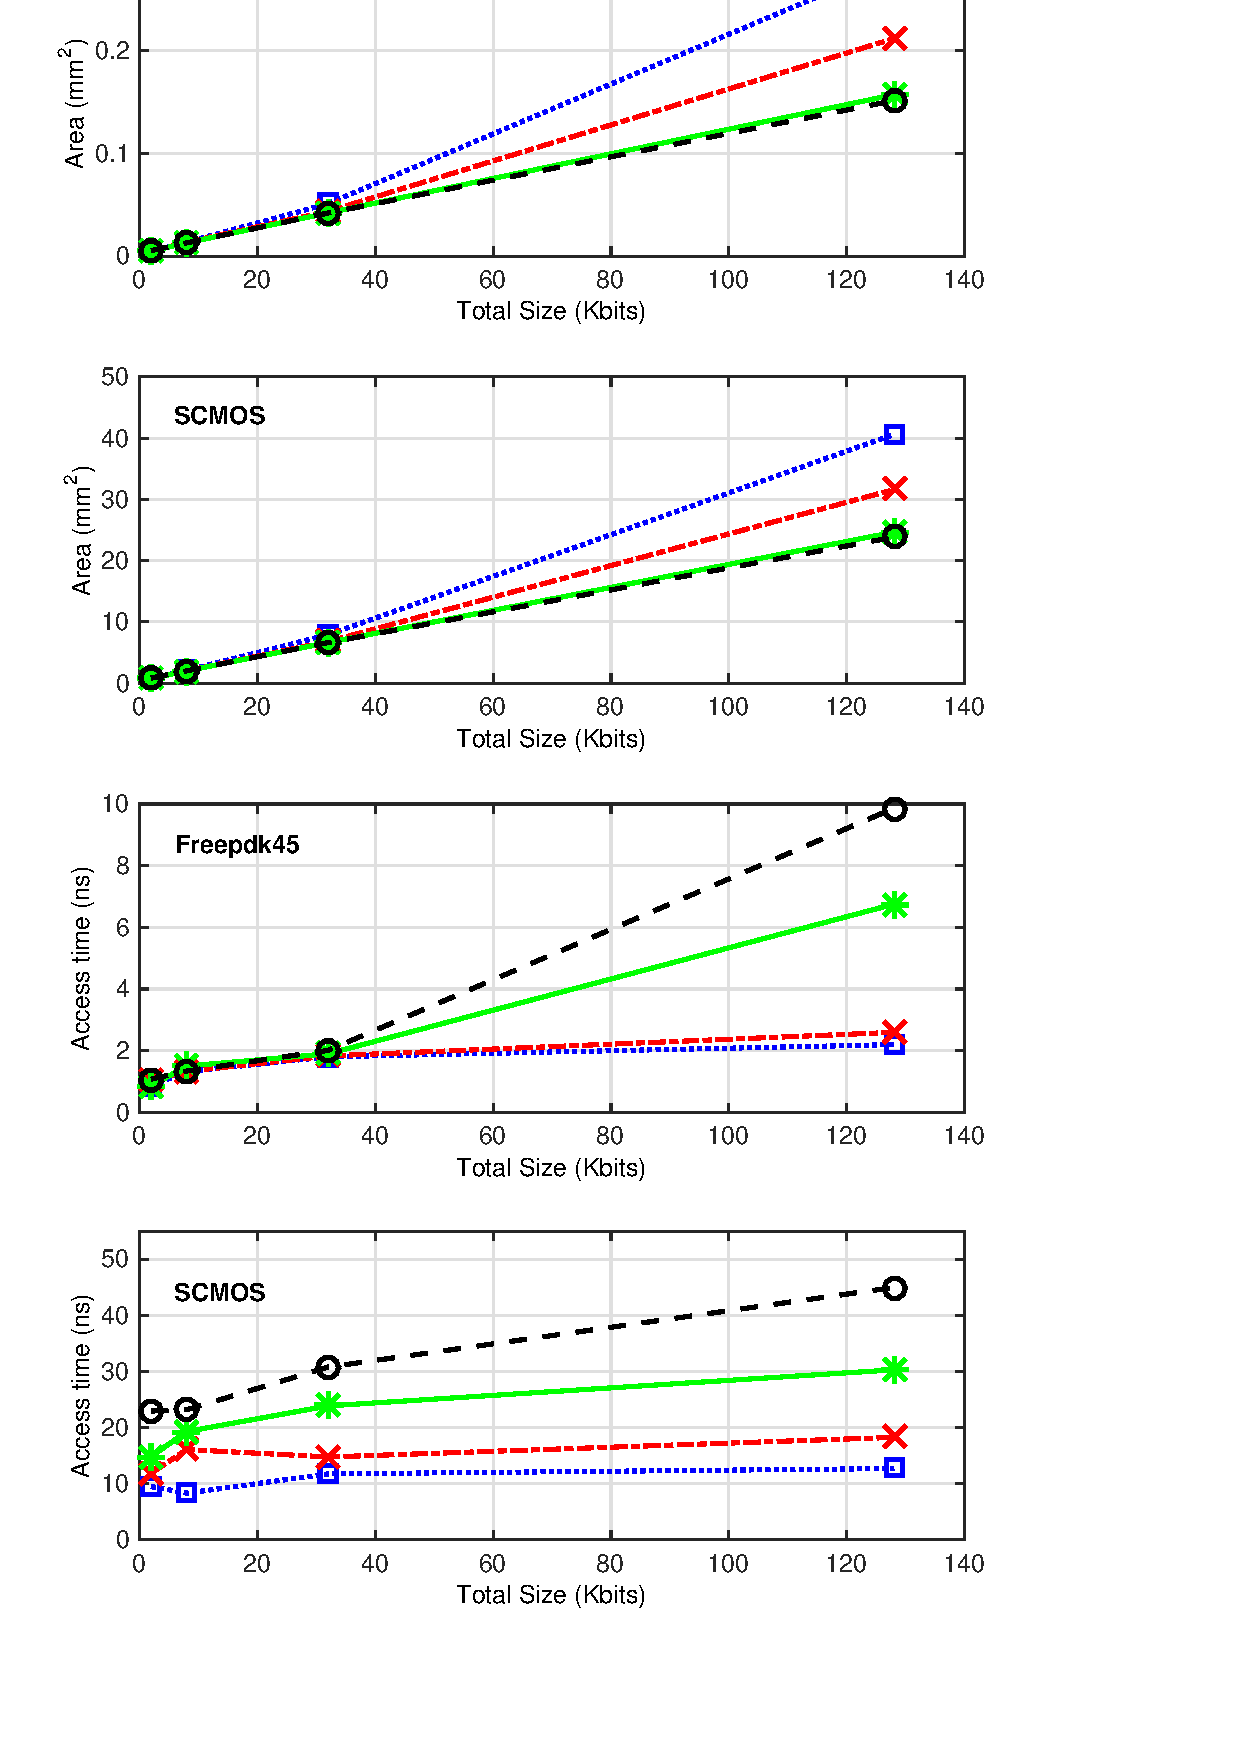
\includegraphics[width=7.5cm , height=14cm]{./figs/Results2.pdf}
%  \subfigure[FreePDK45 memory area \label{fig:freepdk_area}]{
%  \includegraphics[scale=1]{./figs/Freepdk_Area.pdf}}
%  \subfigure[SCMOS memory area \label{fig:scn3me_area}]{
%  \includegraphics[scale=.5]{./figs/Scn3me_Area.pdf}}
  \caption{OpenRAM provides high-density memories in multiple
    technologies and sizes with corresponding characterized
    delays. \label{fig:density_figure}}
  \vspace{-0.5cm}
\end{center}
\end{figure}

%Table~\ref{table:bit-density-comparison} shows a comparison between bit
%density of OpenRAM's generated memory designs and other publications
%which are close in technology node with FreePDK45 and SCMOS. As shown
%in this table, OpenRAM provides very dense SRAM arrays in both technologies.

\begin{table}[t]
\centering
\caption{OpenRAM has high density compared to other published memories in
  similar technologies.}
\begin{tabular}{|c|c|c|c|l|l|l|l|l|} \hline
\texttt{Ref.} & \texttt{Feature} & \texttt{Tech.} & \texttt{Density} \\
                   & \texttt{Size}    &               & [Mb/$mm^2$] \\
\hline \hline
$~\cite{4585946}$       & $65$ nm  & CMOS      & $0.7700$ \\ \hline
$~\cite{Bit_Density_3}$ & $45$ nm  & CMOS      & $0.3300$ \\ \hline
$~\cite{Bit_Density_2}$ & $40$ nm  & CMOS      & $0.9400$ \\ \hline
\verb+OpenRAM+          & $45$ nm  & FreePDK45 & $0.8260$ \\ \hline \hline
$~\cite{127339}$        & $0.5$ um & CMOS      & $0.0036$ \\ \hline
$~\cite{Bit_Density_6}$ & $0.5$ um & BiCMOS    & $0.0020$ \\ \hline
$~\cite{Bit_Density_5}$ & $0.5$ um & CMOS      & $0.0050$ \\ \hline
\verb+OpenRAM+          & $0.5$ um & SCMOS     & $0.0050$ \\ \hline
\end{tabular}
\label{table:bit-density-comparison}
\end{table}

%\begin{table*}
%\centering
%\caption{OpenRAM has high density, fast access time and low power consumption compared to other published memories in similar technologies.}
%\begin{tabular}{|c|l|l|l|l|l|l|l|l|} \hline
%\texttt{Reference} & \texttt{Technology} & \texttt{Density (Mb/$mm^2$)}& \texttt{Access time (ns)}& \texttt{Power consumption} \\ \hline \hline
%$~\cite{Bit_Density_1}$ & $65 nm CMOS$ & $0.77$ & $28$ & $22$ $uW/MHz$ \\ \hline
%$~\cite{Bit_Density_2}$ & $40 nm CMOS$ & $0.94$ & $45$ & $13.8$ $pJ/access/Mbit$ \\ \hline
%$OpenRAM$ & $45 nm FreePDK45$ & $0.826$ & $9.86$ & $13.14$ $mW$ \\ \hline \hline
%$~\cite{Bit_Density_4}$ & $0.5 um CMOS$ & $0.0036$ & $1.5$ & $6$ $W$ \\ \hline
%$~\cite{Bit_Density_6}$ & $0.5 um BiCMOS$ & $0.002$ & $1.5$ & $35$ $W$ \\ \hline
%$~\cite{Bit_Density_5}$ & $0.5 um CMOS$ & $0.005$ & $75$ & $3.9$ $mW$ \\ \hline
%$OpenRAM$ & $0.5 um SCMOS$ & $0.005$ & $44.9$ & $115$ $mW$ \\ \hline
%\end{tabular}
%\label{table:bit-density-comparison}
%\end{table*}

Comparison of power consumption and read access time of different
memories is a bit more complicated to make a conclusion, because there
are many trade-offs. Power and performance are highly dependent on
circuit style (CMOS, ECL, etc.), memory organization (more banks is
faster but sacrifices density), and the optimization goal: low-power
or high-performance.  In general, OpenRAM has reasonable trade-off
between the two and can be customized by using an alternate sense
amplifiers, decoders, or overall dimensional organization.
Table~\ref{table:bit-density-comparison} compares the bit-density of
OpenRAM against published designs using similar technology nodes. The
results show the benefit of technology scaling and that OpenRAM has
very good density in both technologies.  As a comparison, a 76ns SRAM
consumes 3.9mW~\cite{Bit_Density_5} while OpenRAM is much faster at
44.9ns but consumes 115mW for the same size. 

%Table~\ref{table:bit-density-comparison} shows a comparison between bit density, access
%time and power consumption of OpenRAM’s generated mem-
%ory designs and other publications which are close in tech-
%nology node with FreePDK45 and SCMOS. As shown in this
%table, OpenRAM provides very dense SRAM arrays in both
%technologies. There is no easy comparison on power con-
%sumption and read access time as these values vary with the
%array size and configuration. Therefore, we only try to com-
%pare the features of each work from a more general point of
%view.




\section{Conclusions}
\label{sec:conclusions}
This paper introduced OpenRAM, an open-source and portable memory
compiler. OpenRAM generates the circuit, functional model, and layout
of variable-sized SRAMs. In addition, a memory characterizer
provides synthesis timing/power models.

The main motivation behind OpenRAM is to promote and simplify
memory-related research in academia. Since OpenRAM is open-sourced,
flexible, and portable, this memory compiler can be adapted to various
technologies and is easily modified to address specific design
requirements. Therefore, OpenRAM provides a platform to implement and test
new memory designs.

Designs are currently being fabricated to test designs using the
OpenRAM framework in SCMOS. We are also continuously introducing new
features, such as non-6T memories, variability characterization,
word-line segmenting, characterization speed-up, and a graphical user
interface (GUI). We hope to engage an active community in the future
development of OpenRAM.


\section{Acknowledgments}
\label{sec:acknowledgements}
This material is based upon work supported by the National Science
Foundation under Grant No. CNS-1205685 and CNS-1205493. Many students
have contributed to the project throughout their studies including
Jeff Butera, Tom Golubev, Seokjoong Kim, Matthew Gaalswyk, and Son
Bui.


\bibliographystyle{abbrv}
\bibliography{references} % Create bibliography using the file: references.bib

%\input{appendix}
\end{document}
